\documentclass[aspectratio=169]{beamer}

% Research-centric theme
\usetheme{Madrid}
\usecolortheme{beaver}

% Packages
\usepackage[utf8]{inputenc}
\usepackage[T1]{fontenc}
\usepackage{amsmath,amssymb,amsthm}
\usepackage{graphicx}
\usepackage{subcaption}
\usepackage{booktabs}
\usepackage{multirow}
\usepackage{listings}
\usepackage{xcolor}
\usepackage{hyperref}
\usepackage{tikz}
\usepackage{pgfplots}
\pgfplotsset{compat=1.18}

% Code highlighting
\lstset{
    language=OCaml,
    basicstyle=\ttfamily\footnotesize,
    keywordstyle=\color{blue},
    commentstyle=\color{green!60!black},
    stringstyle=\color{red},
    numbers=left,
    numberstyle=\tiny,
    frame=single,
    breaklines=true,
    captionpos=b
}

% Title information
\title[MCAS vs Double-Collect]{Multi-Word Compare-and-Swap: \\ Performance Trade-offs in Atomic Snapshots}
\subtitle{A Comparative Analysis of Synchronization Primitives}
\author{Kunal}
\institute{Department of Computer Science}
\date{April 27, 2026}

\begin{document}

\begin{frame}
    \titlepage
\end{frame}

\begin{frame}{Research Question}
    \begin{block}{Core Research Question}
        \centering
        \Large
        \textbf{Does MCAS provide enough expressive power to meaningfully simplify the implementation of an atomic snapshot object, and what is the performance cost of the software MCAS layer?}
    \end{block}

    \vspace{0.5cm}

    \begin{itemize}
        \item \textbf{MCAS}: Multi-Word Compare-and-Swap primitive
        \item \textbf{Atomic Snapshot}: Concurrent data structure for consistent reads
        \item \textbf{Double-Collect}: Baseline algorithm from previous assignment
    \end{itemize}
\end{frame}

\begin{frame}{Background: Atomic Snapshots}
    \begin{columns}[c]
        \column{0.6\textwidth}
        \begin{itemize}
            \item \textbf{Problem}: Need consistent view of multiple shared registers
            \item \textbf{Challenge}: Hardware only provides single-word CAS
            \item \textbf{Solution}: Software-based multi-word operations
        \end{itemize}

        \vspace{0.3cm}
        \begin{block}{Operations}
            \begin{itemize}
                \item \texttt{update(i, v)}: Write value \texttt{v} to register \texttt{i}
                \item \texttt{scan()}: Return consistent snapshot of all registers
            \end{itemize}
        \end{block}

        \column{0.4\textwidth}
        \begin{figure}
            \centering
            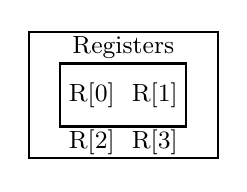
\begin{tikzpicture}[scale=0.8]
                \draw[thick] (0,0) rectangle (3,2);
                \draw[thick] (0.5,1.5) -- (2.5,1.5) -- (2.5,0.5) -- (0.5,0.5) -- cycle;
                \node at (1.5,1.75) {\small Registers};
                \node at (1,1) {\small R[0]};
                \node at (2,1) {\small R[1]};
                \node at (1,0.25) {\small R[2]};
                \node at (2,0.25) {\small R[3]};
            \end{tikzpicture}
            \caption{Atomic snapshot data structure}
        \end{figure}
    \end{columns}
\end{frame}

\begin{frame}{Implementation 1: Double-Collect Algorithm}
    \begin{columns}[c]
        \column{0.5\textwidth}
        \begin{block}{Algorithm Overview}
            \begin{enumerate}
                \item Collect all register values
                \item Collect again immediately
                \item If values match, return them
                \item Otherwise, retry
            \end{enumerate}
        \end{block}

        \vspace{0.3cm}
        \begin{block}{Key Properties}
            \begin{itemize}
                \item Only uses atomic reads
                \item No modifications during scan
                \item Simple and efficient
            \end{itemize}
        \end{block}

        \column{0.5\textwidth}
        \begin{lstlisting}[caption=Double-Collect Scan]
let rec scan snapshot =
  let c1 = collect snapshot in
  let c2 = collect snapshot in
  if c1 = c2 then c1
  else scan snapshot
        \end{lstlisting}
    \end{columns}
\end{frame}

\begin{frame}{Implementation 2: MCAS-Based Snapshot}
    \begin{columns}[c]
        \column{0.5\textwidth}
        \begin{block}{Algorithm Overview}
            \begin{enumerate}
                \item Read current values
                \item Create MCAS operations to validate consistency
                \item Execute MCAS atomically
                \item Retry if validation fails
            \end{enumerate}
        \end{block}

        \vspace{0.3cm}
        \begin{block}{Key Properties}
            \begin{itemize}
                \item Uses multi-word CAS primitive
                \item Stronger atomicity guarantees
                \item More complex implementation
            \end{itemize}
        \end{block}

        \column{0.5\textwidth}
        \begin{lstlisting}[caption=MCAS-Based Scan]
let rec scan t =
  let snapshot = Array.map get t.slots in
  let ops = Array.mapi (fun i value ->
    make_cas t.slots.(i) ~expected:value ~desired:value
  ) snapshot in
  if mcas ops then snapshot else scan t
        \end{lstlisting}
    \end{columns}
\end{frame}

\begin{frame}{Benchmark Setup}
    \begin{columns}[c]
        \column{0.6\textwidth}
        \begin{block}{Experimental Parameters}
            \begin{itemize}
                \item \textbf{Registers}: 16 atomic registers
                \item \textbf{Threads}: 2, 4, 8, 16, 32 domains
                \item \textbf{Operations}: 20,000 per domain
                \item \textbf{Workloads}:
                    \begin{itemize}
                        \item 100\% updates
                        \item 50\% updates / 50\% scans
                        \item 10\% updates / 90\% scans
                        \item 100\% scans
                    \end{itemize}
            \end{itemize}
        \end{block}

        \column{0.4\textwidth}
        \begin{figure}
            \centering
            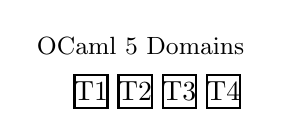
\begin{tikzpicture}[scale=0.7]
                \foreach \i in {1,...,4} {
                    \draw[thick] (\i*0.8,0) rectangle (\i*0.8+0.6,0.6);
                    \node at (\i*0.8+0.3,0.3) {T\i};
                }
                \node[above] at (2,0.8) {\small OCaml 5 Domains};
            \end{tikzpicture}
            \caption{Multi-domain execution}
        \end{figure}
    \end{columns}
\end{frame}

\begin{frame}{Benchmark Results: Overview}
    \begin{figure}
        \centering
        
\includegraphics[width=\textwidth,height=0.7\textheight,keepaspectratio]{assets/benchmark_overview.png}
        \caption{Elapsed time comparison across all workloads and thread counts}
    \end{figure}
\end{frame}

\begin{frame}{Benchmark Results: Relative Performance}
    \begin{columns}[c]
        \column{0.6\textwidth}
        \begin{figure}
            \centering
            
\includegraphics[width=\textwidth,height=0.6\textheight,keepaspectratio]{assets/relative_to_baseline.png}
            \caption{MCAS slowdown relative to double-collect baseline}
        \end{figure}

        \column{0.4\textwidth}
        \begin{block}{Key Observations}
            \begin{itemize}
                \item MCAS consistently slower
                \item Scan-heavy workloads hit hardest
                \item Performance gap grows with threads
            \end{itemize}
        \end{block}
    \end{columns}
\end{frame}

\begin{frame}{Workload Analysis: 100\% Updates}
    \begin{figure}
        \centering
        
\includegraphics[width=\textwidth,height=0.7\textheight,keepaspectratio]{assets/updates_100.png}
        \caption{Performance comparison for update-only workloads}
    \end{figure}

    \begin{block}{Analysis}
        Even for update-heavy workloads, MCAS introduces overhead due to the software CAS layer and descriptor management.
    \end{block}
\end{frame}

\begin{frame}{Workload Analysis: Balanced 50/50}
    \begin{figure}
        \centering
        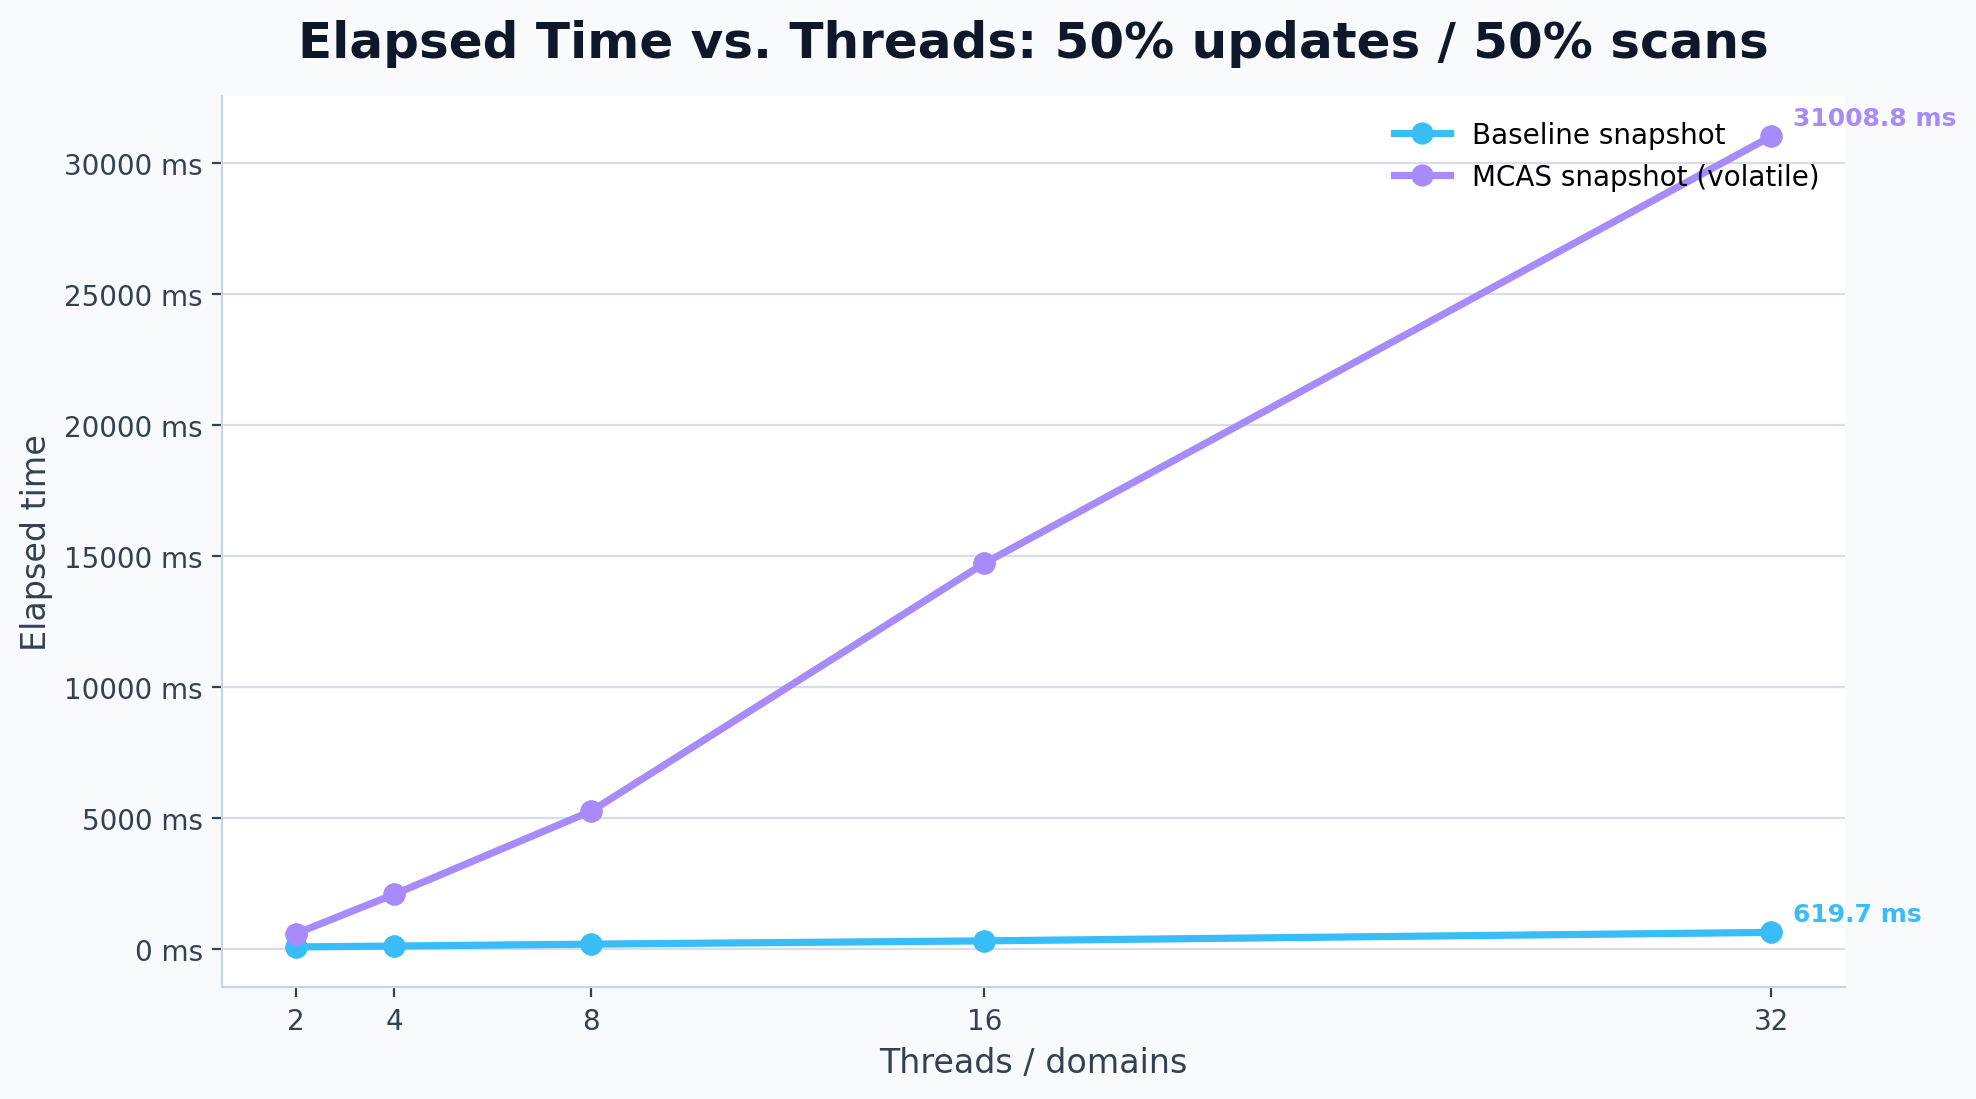
\includegraphics[width=\textwidth,height=0.7\textheight,keepaspectratio]{assets/balanced_50_50.png}
        \caption{Performance comparison for mixed workloads}
    \end{figure}

    \begin{block}{Analysis}
        Mixed workloads show moderate performance degradation. The MCAS layer adds latency to both update and scan operations.
    \end{block}
\end{frame}

\begin{frame}{Workload Analysis: Scan-Heavy Workloads}
    \begin{columns}[c]
        \column{0.5\textwidth}
        \begin{figure}
            \centering
            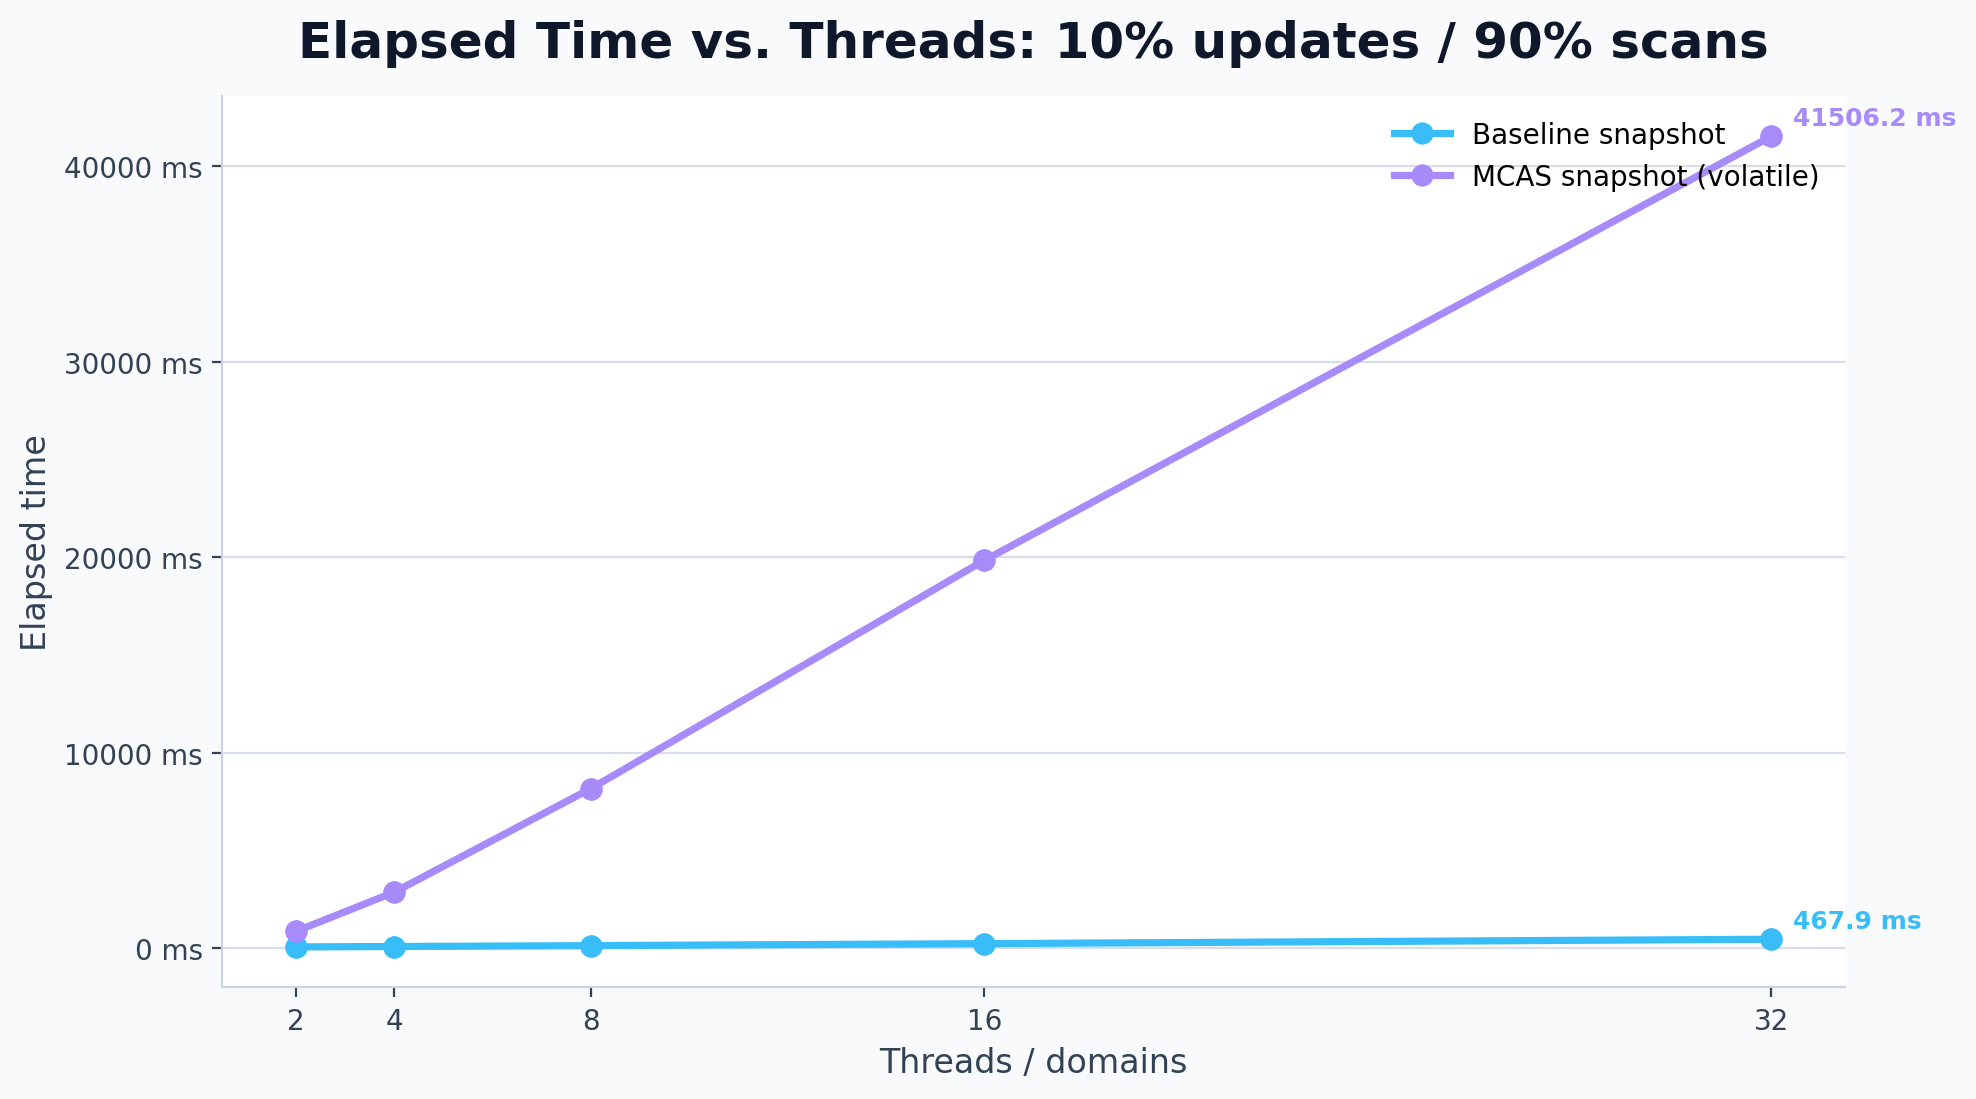
\includegraphics[width=\textwidth,height=0.8\textheight,keepaspectratio]{assets/scans_90.png}
            \caption{10\% updates / 90\% scans}
        \end{figure}

        \column{0.5\textwidth}
        \begin{figure}
            \centering
            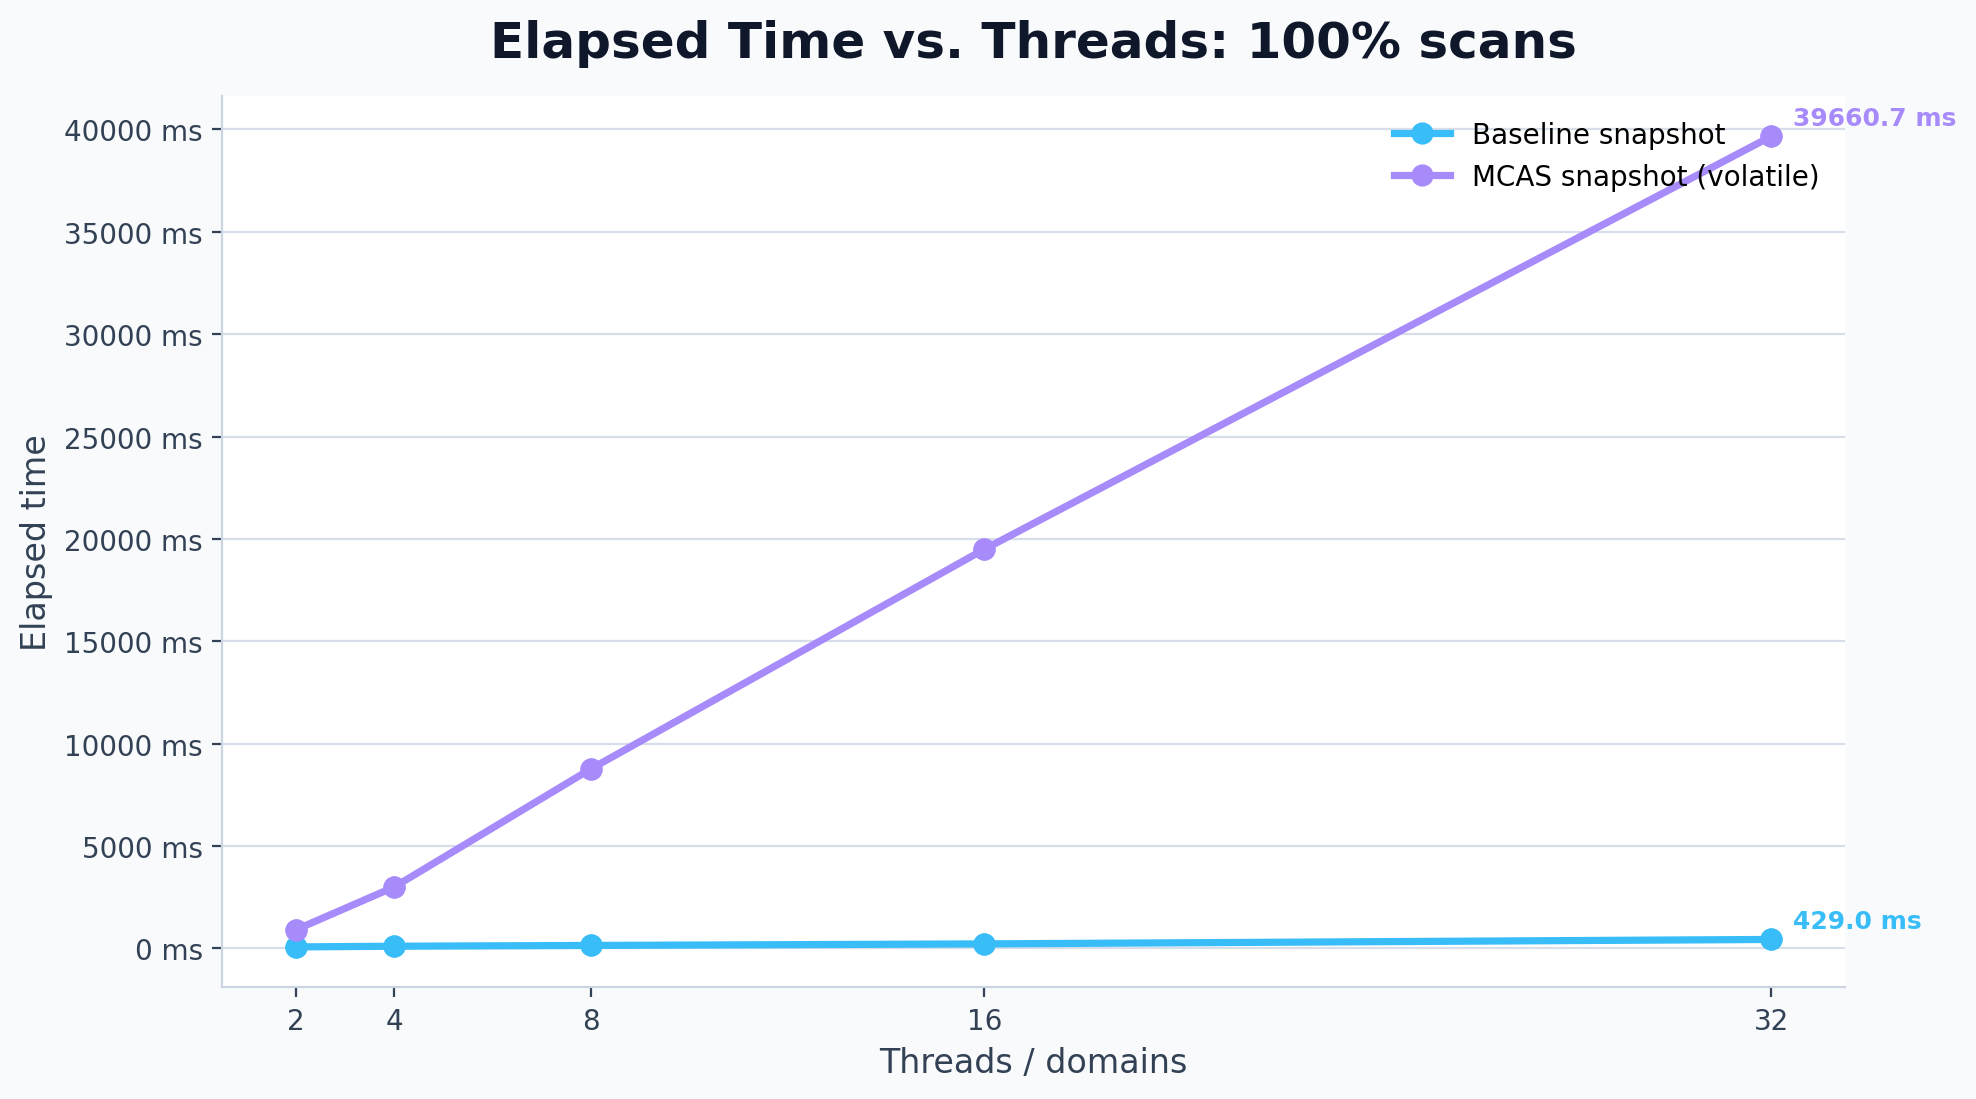
\includegraphics[width=\textwidth,height=0.8\textheight,keepaspectratio]{assets/scans_100.png}
            \caption{100\% scans}
        \end{figure}
    \end{columns}
\end{frame}

\begin{frame}{The Performance Trade-off}
    \begin{block}{Why is MCAS Slower?}
        \begin{itemize}
            \item \textbf{Double-Collect}: Only atomic reads, no modifications
            \item \textbf{MCAS}: Full multi-word CAS operation for validation
            \item \textbf{Overhead}: Descriptor creation, helping mechanisms, RDCSS
        \end{itemize}
    \end{block}

    \vspace{0.3cm}

    \begin{block}{What Does MCAS Provide?}
        \begin{itemize}
            \item \textbf{Expressiveness}: Uniform implementation of updates and scans
            \item \textbf{Composability}: Can build complex atomic operations
            \item \textbf{Correctness}: Stronger atomicity guarantees
        \end{itemize}
    \end{block}
\end{frame}

\begin{frame}{Quantitative Analysis}
    \begin{table}
        \centering
        \begin{tabular}{@{}lcccc@{}}
            \toprule
            Workload & Threads & Double-Collect & MCAS & Slowdown \\
            \midrule
            100\% Updates & 32 & 0.088 μs/op & 0.194 μs/op & 2.2x \\
            50/50 Mixed & 32 & 0.172 μs/op & 4.724 μs/op & 27.5x \\
            10\% Updates & 32 & 0.153 μs/op & 6.137 μs/op & 40.1x \\
            100\% Scans & 32 & 0.118 μs/op & 6.29 μs/op & 53.3x \\
            \bottomrule
        \end{tabular}
        \caption{Average time per operation at 32 threads (from latest benchmark)}
    \end{table}

    \begin{block}{Key Insight}
        The performance cost is workload-dependent: scan operations suffer the most because MCAS validation requires modifying all registers atomically.
    \end{block}
\end{frame}

\begin{frame}{Implementation Complexity Comparison}
    \begin{columns}[c]
        \column{0.5\textwidth}
        \begin{block}{Double-Collect}
            \begin{itemize}
                \item Simple algorithm
                \item Few lines of code
                \item Easy to understand
                \item Limited to snapshots
            \end{itemize}
        \end{block}

        \column{0.5\textwidth}
        \begin{block}{MCAS-Based}
            \begin{itemize}
                \item Complex descriptor system
                \item Helping mechanisms
                \item RDCSS primitives
                \item Reusable for other structures
            \end{itemize}
        \end{block}
    \end{columns}

    \vspace{0.3cm}
    \begin{block}{Trade-off Summary}
        \textbf{Simplicity vs. Expressiveness}: Double-collect is fast and simple but limited. MCAS is slower but provides a powerful primitive for building complex concurrent data structures.
    \end{block}
\end{frame}

\begin{frame}{Conclusion}
    \begin{block}{Answering the Research Question}
        \begin{itemize}
            \item \textbf{Expressiveness}: MCAS does simplify atomic snapshot implementation by providing a uniform abstraction for both updates and scans
            \item \textbf{Performance Cost}: Significant overhead, especially for read-heavy workloads (up to 53x slower for pure scans)
            \item \textbf{Trade-off}: Choose based on requirements - performance vs. composability
        \end{itemize}
    \end{block}

    \vspace{0.3cm}

    \begin{block}{Key Takeaways for Students}
        \begin{itemize}
            \item Software synchronization primitives have inherent costs
            \item Stronger guarantees often come with performance trade-offs
            \item Choose the right tool for the job - sometimes simple algorithms outperform complex ones
        \end{itemize}
    \end{block}
\end{frame}

\begin{frame}{Questions?}
    \begin{center}
        \Huge Questions?
    \end{center}

    \vspace{0.5cm}

    \begin{block}{Further Reading}
        \begin{itemize}
            \item Harris, Fraser, Pratt: "A Practical Multi-Word Compare-and-Swap Operation"
            \item Guerraoui et al.: "Efficient Multi-word Compare and Swap"
            \item OCaml 5 Multicore Documentation
        \end{itemize}
    \end{block}
\end{frame}

\end{document}